\documentclass[twocolumn]{article}
\usepackage{amsmath}
\usepackage{amssymb}
\usepackage{graphicx}

\begin{document}
\section{The Assignment}

\subsection{Time Dependent PDEs}

In this section, we begin exploring time-dependent partial
differential equations, specifically building up to the
advection-diffusion equation by considering each case individually
first, then combining them into one equation. We will also test
different explicit and implicit finite differencing schemes to step
forward in time and test the Courant-Fiedrichs-Lewy (CFL) condition,
which is usually used to determine the size of the time step.

\subsubsection{The Advection Equation}

The one-dimensional advection equation is a function of
concentration $u(t, x)$ over time:
\begin{equation}
  u_t = c u_x
\end{equation}
where $c$ is the speed of flow. In a similar vein to d'Alembert's
solution to the wave equation, the exact solution to the 1D advection
equation is found by shifting the initial conditions, $u(0, x)$, along
the $x$-axis:
\begin{equation}
  u(t, x) = u(0, x + ct)
\end{equation}
This means that if $c$ is positive, the initial function is shifted to
the left. The opposite is true if $c$ is negative, the initial
function is shifted to the right.

To find a numerical solution to the advection equation, we applied
four different finite difference schemes: forward and backward Euler,
Lax-Wendroff, and Crank-Nicholson. These four schemes will be used on
four different initial conditions, shown in table \ref{table:cases}
with seven different sets of parameters, shown in table
\ref{table:advection}. The value $r$ is the Courant number, which is a
result of the CFL condition. This is a way to determing the stability
of the system. Generally, the Courant number is set to be less than
one for the system to be stable.

\begin{table}
\begin{centering}
\begin{tabular}{c|c}
  Case & Function \\ \hline \hline
  0    & $u(0, x) = \sin(2 x)$ \\ \hline
  1    & $u(0, x) = \begin{cases} 0 & \text{if} \; x < 0 \\ 1 &
    \text{if} \; x \geq 0 \end{cases}$ \\ \hline
  2    & $u(0, x) = \delta_{x, 0} / \Delta x$ \\ \hline
  3    & $\exp(- 4 x^2)$
\end{tabular}
\caption{The initial conditions for the advection equation.}
\label{table:cases}
\end{centering}
\end{table}

\begin{table}
\begin{centering}
\begin{tabular}{c|c|c|c|c}
  Trial & $c$ & $\Delta x$ & $\Delta t$ & $r = c \Delta t / \Delta x$ \\ \hline \hline
  0     & 0.5 & 0.04       & 0.02       & 0.25                        \\ \hline
  1     & 0.5 & 0.02       & 0.02       & 0.5                         \\ \hline
  2     & 0.5 & 0.0137     & 0.02       & 0.728                       \\ \hline
  3     & 0.5 & 0.0101     & 0.02       & 0.99                        \\ \hline
  4     & 0.5 & 0.0099     & 0.02       & 1.11                        \\ \hline
  5     & 0.5 & 0.02       & 0.01       & 0.25                        \\ \hline
  6     & 0.5 & 0.02       & 0.04       & 1
\end{tabular}
\caption{The sets of parameters used when computing the advection equation.}
\label{table:advection}
\end{centering}
\end{table}

\begin{figure*}[t]
  \centering
  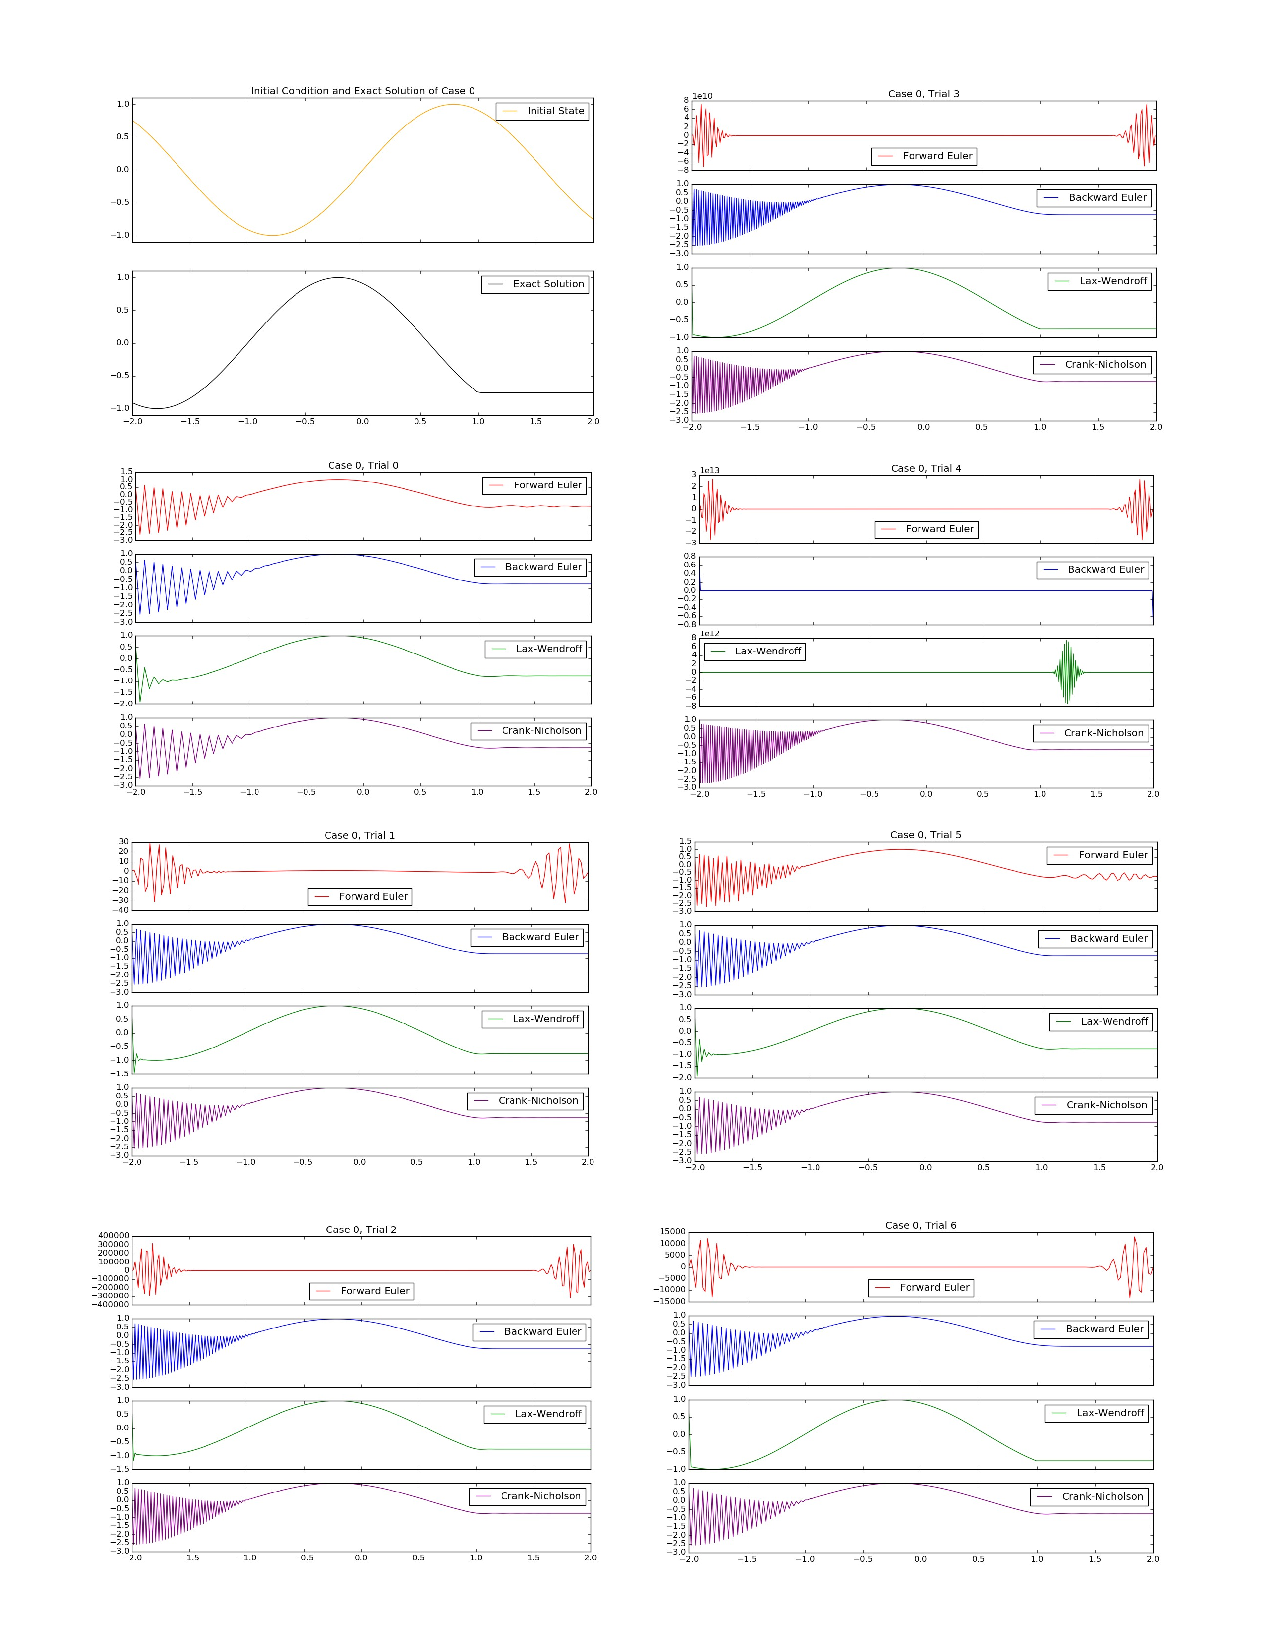
\includegraphics[width=\textwidth]{case0}
  \caption{
    The numerical solution to case $0$ from table \ref{table:cases}
    for seven trials, a simple sinusoid. The initial condition and
    exact solutions are shown in the top left and the solutions are
    are for $t=2$.
  }
  \label{fig:case0}
\end{figure*}

The first case, shown in figure \ref{fig:case0} is a simple
sinusoid. Since the pulse propogates to the left, the right side of
the exact solution remains constant at the value of the boundary. The
first trial, with $r = 0.25$, all methods are able to approximate the
solution, though there are oscillations on the left side due to the
boundary condition. Once $r >= 0.5$, the explicit forward Euler scheme
no longer propogates the initial pulse correctly and flatlines at zero
while the areas around the boundary increase to infinity. The smaller
values of $\Delta x$ also increase the oscillations seen in the
implicit methods. For trial $4$, $r = 1.11$, and all methods become
unstable except for the Crank-Nicholson scheme, which combines the
explicit and implicit Euler methods.

\begin{figure*}
  \centering
  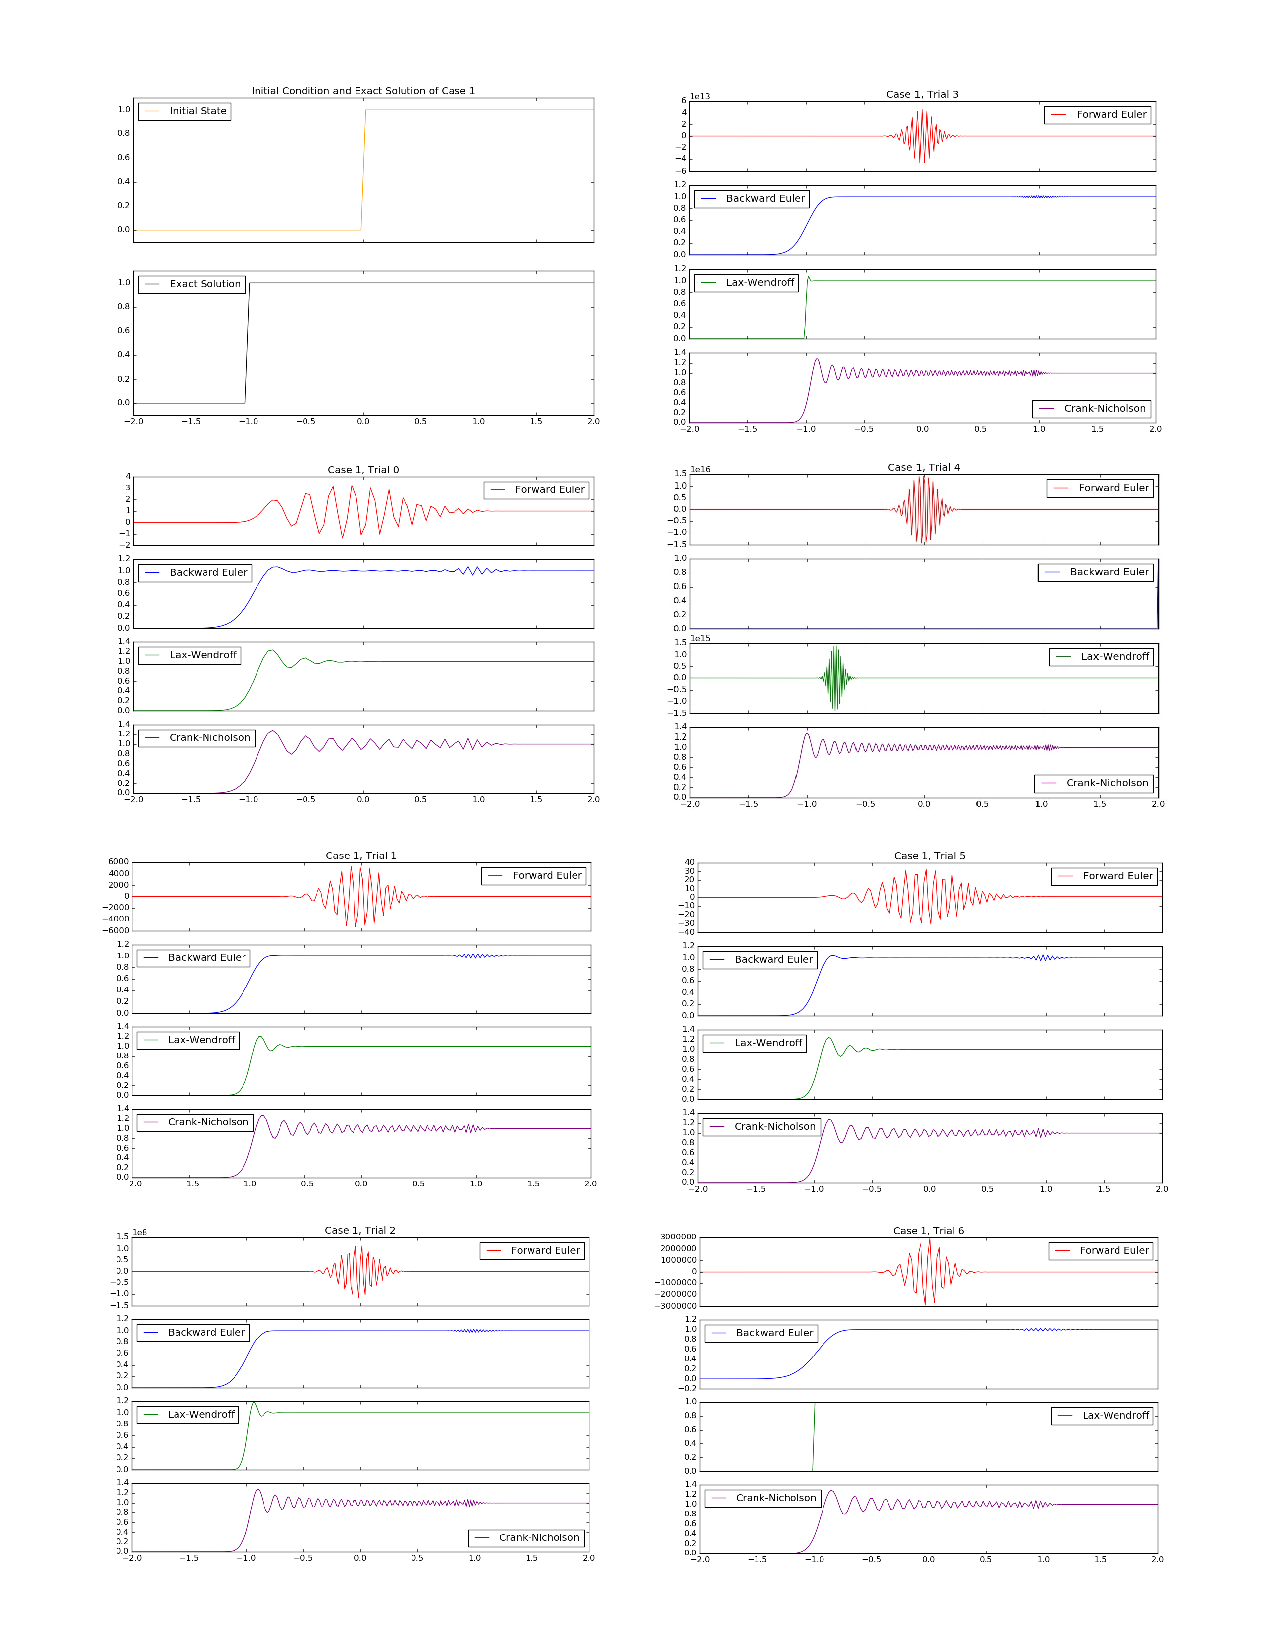
\includegraphics[width=\textwidth]{case1}
  \caption{
    The numerical solution to case $1$, a Heaviside function. The
    initial condition and exact solution are shown in the top left
    corner and the solutions are for $t=2$.
  }
  \label{fig:case1}
\end{figure*}

The second case, shown in figure \ref{fig:case1} is a Heaviside
function centred at $x=0$. Similarly to the first case, the forward
Euler method is the most unstable, unable to approximate the solution
in any of the cases. Trial $4$ also shows once again that the
Crank-Nicholson scheme is the most stable while the other methods lose
their stability once $r >= 1$. However, the explicit Lax-Wendroff
scheme is the most accurate and has the fewest oscillations as $\Delta
x$ decreases.

\begin{figure*}
  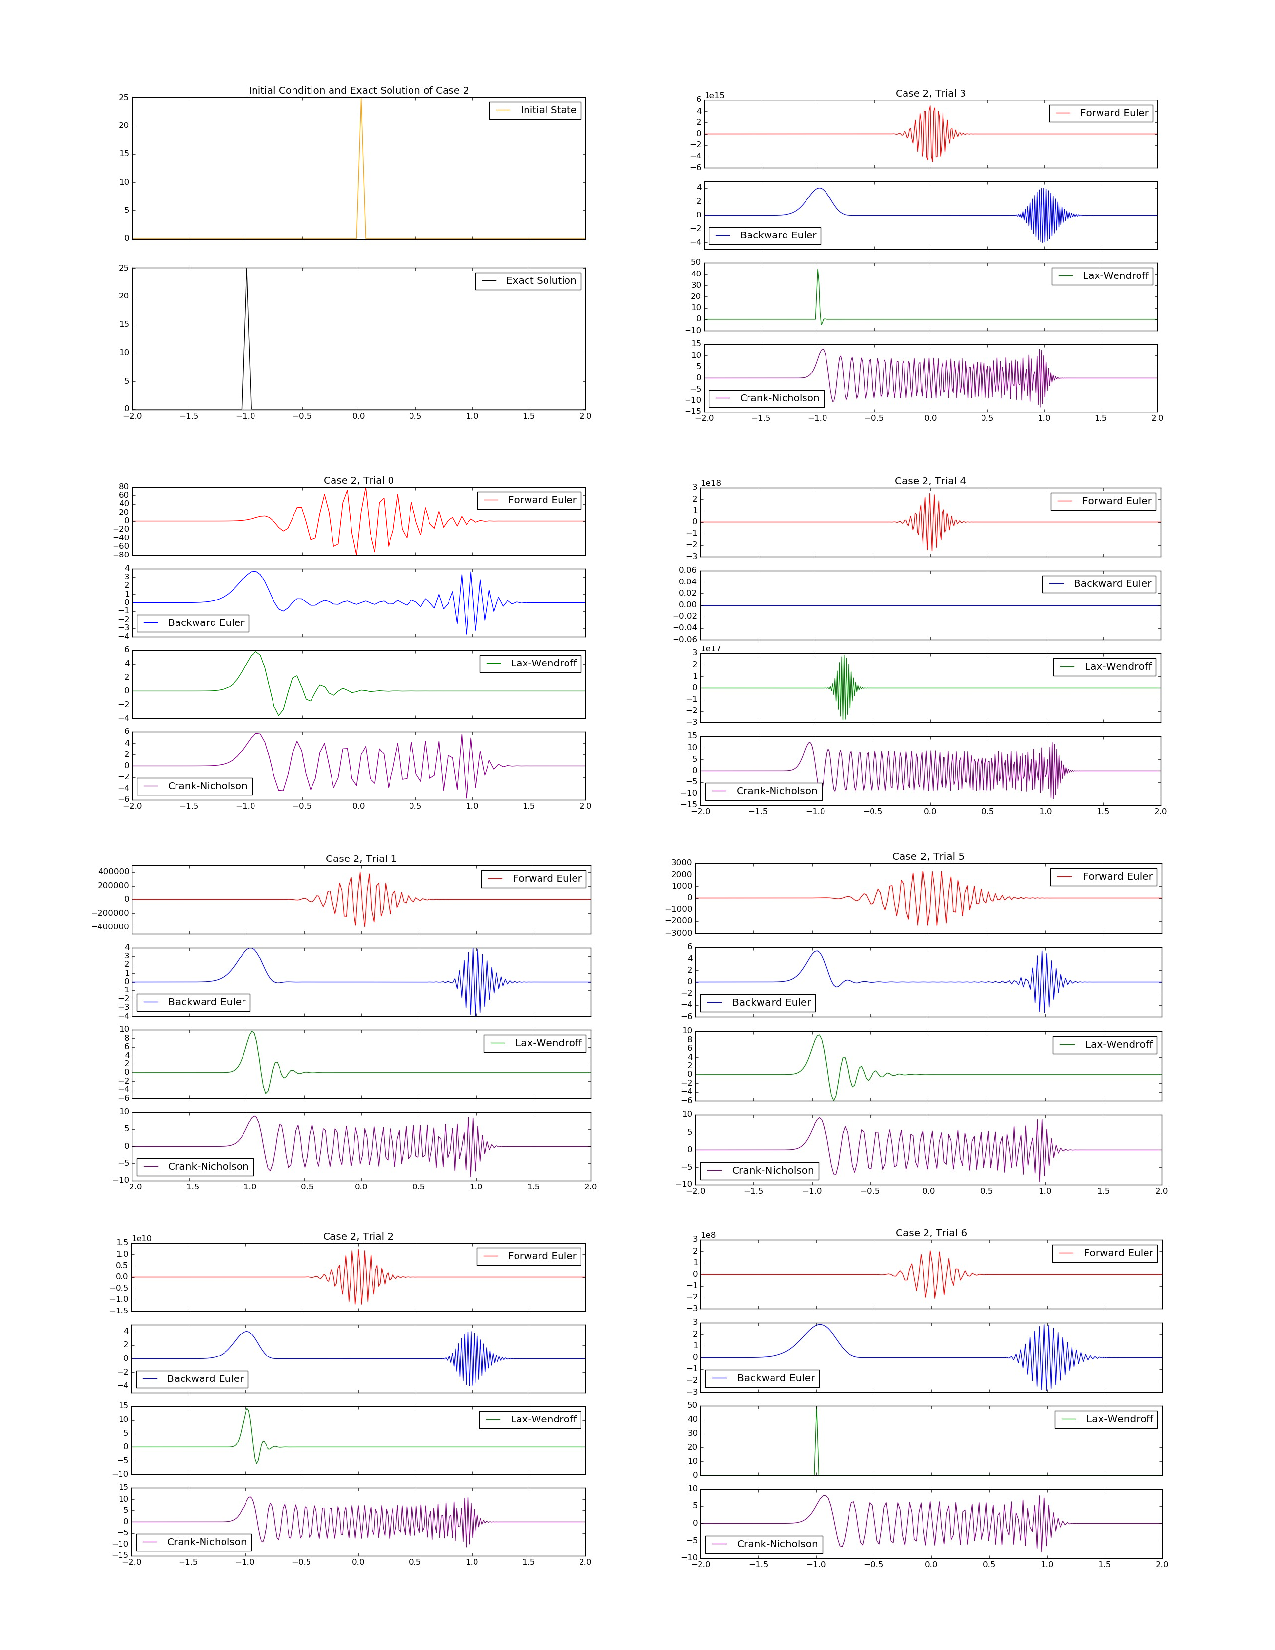
\includegraphics[width=\textwidth]{case2}
  \caption{
    The numerical solution to case $2$, a delta function. The initial
    condition and exact solution are shown in the top left corner and
    the solutions are for $t=2$. It should be noted that the size of
    the pulse is dependent on the value of $\Delta x$ for each trial.
  }
  \label{fig:case2}
\end{figure*}

The third case, shown in figure \ref{fig:case2} is a delta
function. The magnitude of the pulse is dependent on the value $\Delta
x$, and is thus dependent on the parameters defined in the
trial. Regardless of the magnitude of the pulse, it propogates the
same way. Many of the properties seen in the previous case are present
here as well: forward Euler is very unstable, Crank-Nicholson is the
most stable, and Lax-Wendroff gives the most accurate result when the
CFL condition is maintained. The unique aspects of this case are from
the oscillations. In both the backward Euler and Crank-Nicholson
schemes, there is a large oscillation on the other side of where the
actual pulse is. The oscilations in the latter, however, become so
large and numerous that it is difficult to tell where the important
information is and which peaks are noise. This would also imply that
the Crank-Nicholson scheme is very sensitive to sharp spikes in data
while the Lax-Wendroff scheme is able to propogate them better.

\begin{figure*}
  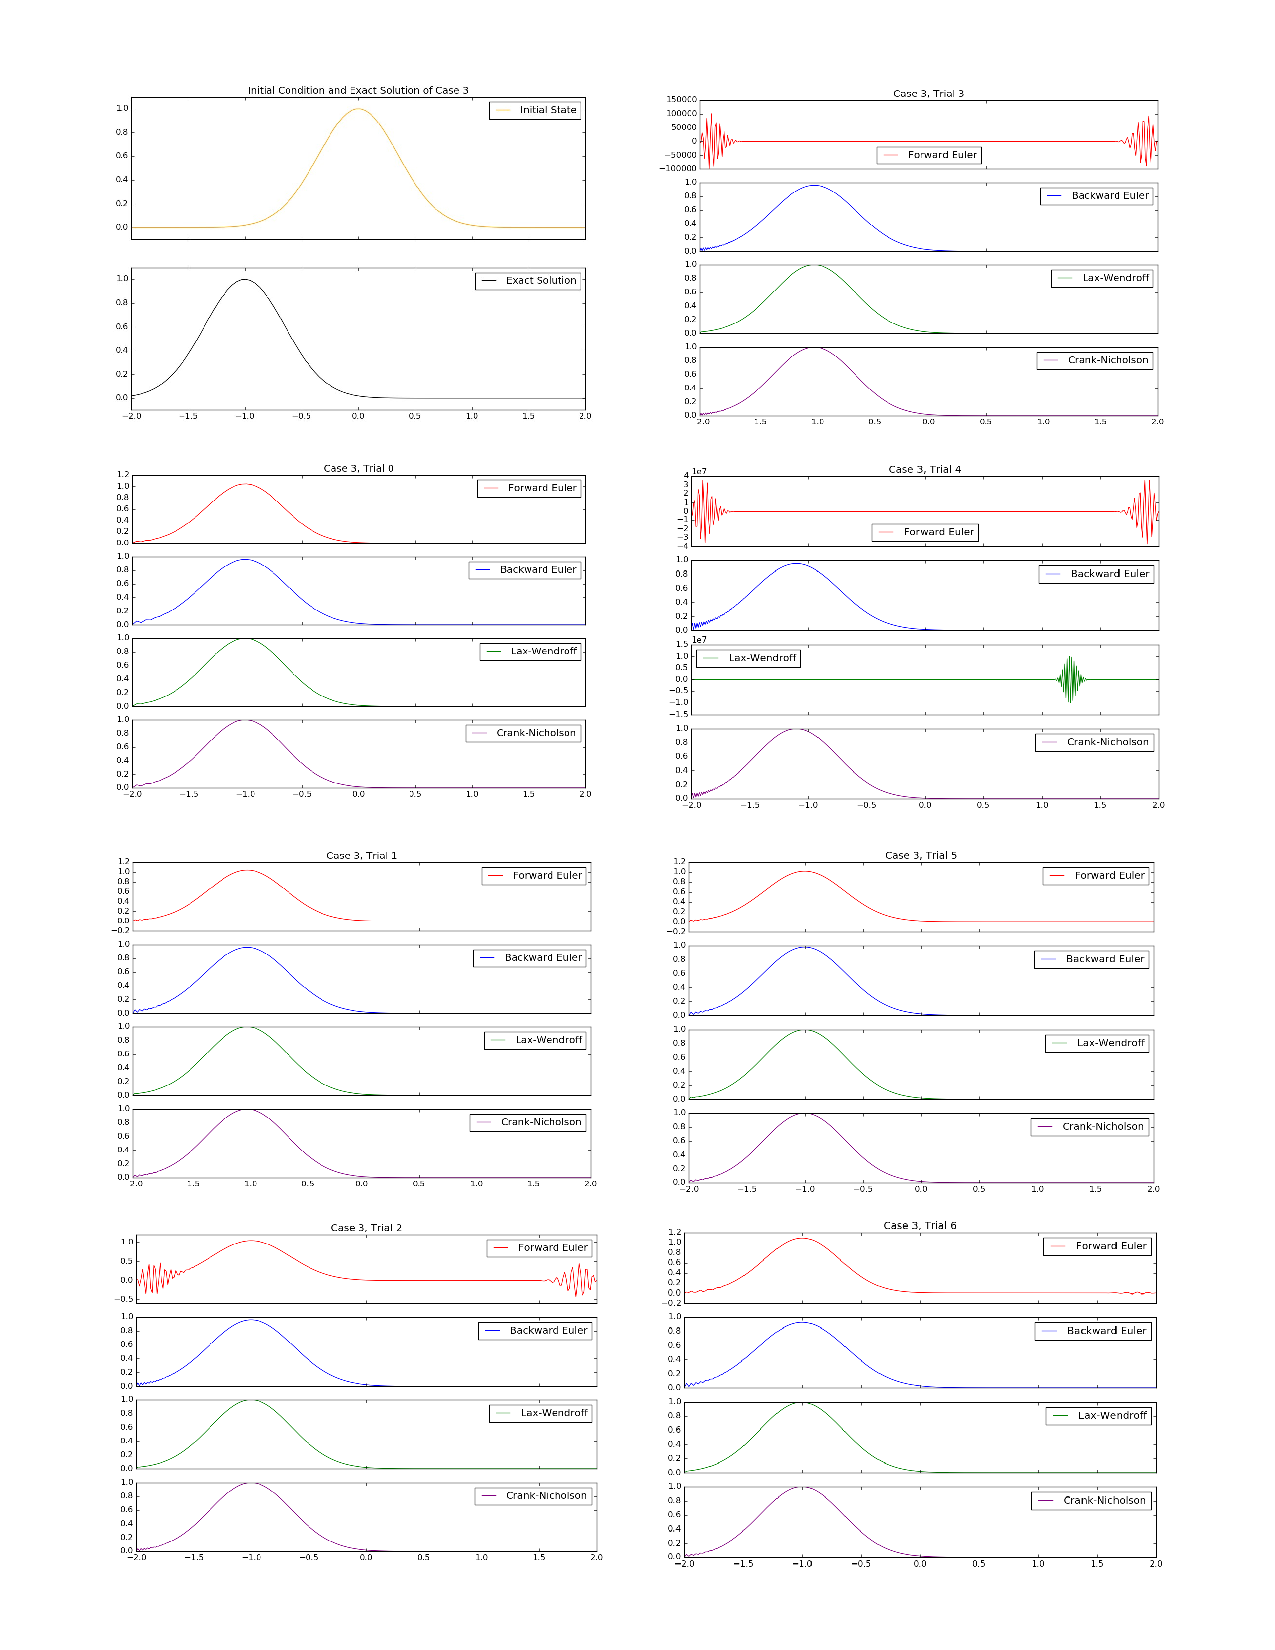
\includegraphics[width=\textwidth]{case3}
  \caption{
    The numerical solution to case $3$, a Gaussian distribution with
    its peak centred about $x=0$. The initial condition and exact
    solution are shown in the top left corner and the solutions are
    for $t=2$.
  }
  \label{fig:case3}
\end{figure*}

The final case we are considering a a Gaussian distribution centred
about $x=0$. Since this case does not have sharp abrupt changes in
slope, all the methods are able to propagate it a little better and
the oscillations present in the implicit methods are greatly reduced.

\subsubsection{The Diffusion Equation}

The pure diffusion equation describes an initial pulse which diffuses into
the surrounding fluid. The one dimensional diffusion equation is:
\begin{equation}
  u_t = \beta u_{xx}
\end{equation}
where $\beta$ is the diffusion coefficient. The exact solution for $x$ over the
interval $\left[0, 1 \right]$ for the initial condition $u(0, x) = \sin(\pi x)$ and
boundary conditions $u(t, 0) = u(t, 1) = 0$ is:
\begin{equation}
  \label{eq:diffusion}
  u(t, x) = e^{- \beta \pi^2 t} \sin(\pi x)
\end{equation}
In order to solve the equation numerically, we can change the diffusion equation
into a FD equation. Replacing the time derivative with a first order forward
difference scheme and the spatial derivative by a centred difference scheme
results in the equation:
\begin{equation}
  u_i^{n+1} = u_i^n + r \left( u_{i+1}^n - 2 u_i^n + u_{i-1}^n \right)
\end{equation}
where the Courant number is $r = \frac{\beta \Delta t}{(\Delta x)^2}$,
  $n$ is along the time axis and $j$ is along the $x$-axis.
The conditions for stability can be found through von Neumann
stability analysis. Starting from the finite difference equation,
stepping forward in time and centred stepping in space:
\begin{equation}
  \frac{u_j^{n+1} - u_j^n}{\Delta t} = \beta \frac{u_{j+1}^n - 2 u_j^n
    + u_{j-1}^n}{\Delta x^2}
\end{equation}
we first assume that the each step can be represented as a product of
an amplification factor $G^n$ and an exponential term so that $u_j^n =
G^n e^{i k j \Delta x}$. This form of $u_j^n$ is then substituted into
the FD equation and solved for $G^1$:
\begin{equation}
  \begin{aligned}
    e^{i k j \Delta x} \frac{G^{n+1} - G^n}{\Delta t} &= \beta G^n
    \frac{e^{i k (j + 1) \Delta x} - 2 e^{i k j \Delta x} + e^{i k (j
        - 1) \Delta x}}{\Delta x^2} \\
    G^1 - 1 &= \frac{\beta \Delta t}{\Delta x^2} \left(e^{- i k \Delta
        x} - 2 + e^{+ i k \Delta x} \right) \\
    \therefore G^1 &= \left( 1 - 2 r \right) + 2 r \cos(k \Delta x)
  \end{aligned}
\end{equation}
where $r = \frac{\beta \Delta t}{\Delta x^2}$ in the last
substitution.

For stability, we impose the condition that $|G^n| \leq 1$. If the
cosine term is equal to one ($\cos(k \Delta x) = 1$), then $|G^n| =
1$, which satisfies the stability condition. However, if the cosine
term is equal to negative one, we use the fact that $r > 0$, so the
stability condition becomes:
\begin{equation}
  \begin{aligned}
    |G^n| &\leq 1 - 4 r \\
    - 1 &\leq 1 - 4 r \\
    \therefore \Delta t &\leq \Delta t_{max} = \frac{\Delta x^2}{2 \beta}
  \end{aligned}
\end{equation}

When the diffusion equation was solved numerically for the conditions
described in equation \ref{eq:diffusion}, it was run for $300$ time
steps, $51$ grid points, $\beta = 1$, and $\Delta t = 0.9 \Delta
t_{max}$, the results shown in figure \ref{fig:diffusion}. Since the
CFL conditions are met, the solution is stable and very closely
approximates the exact solution, though the height of the peak is
slightly overestimated.

\begin{figure}
  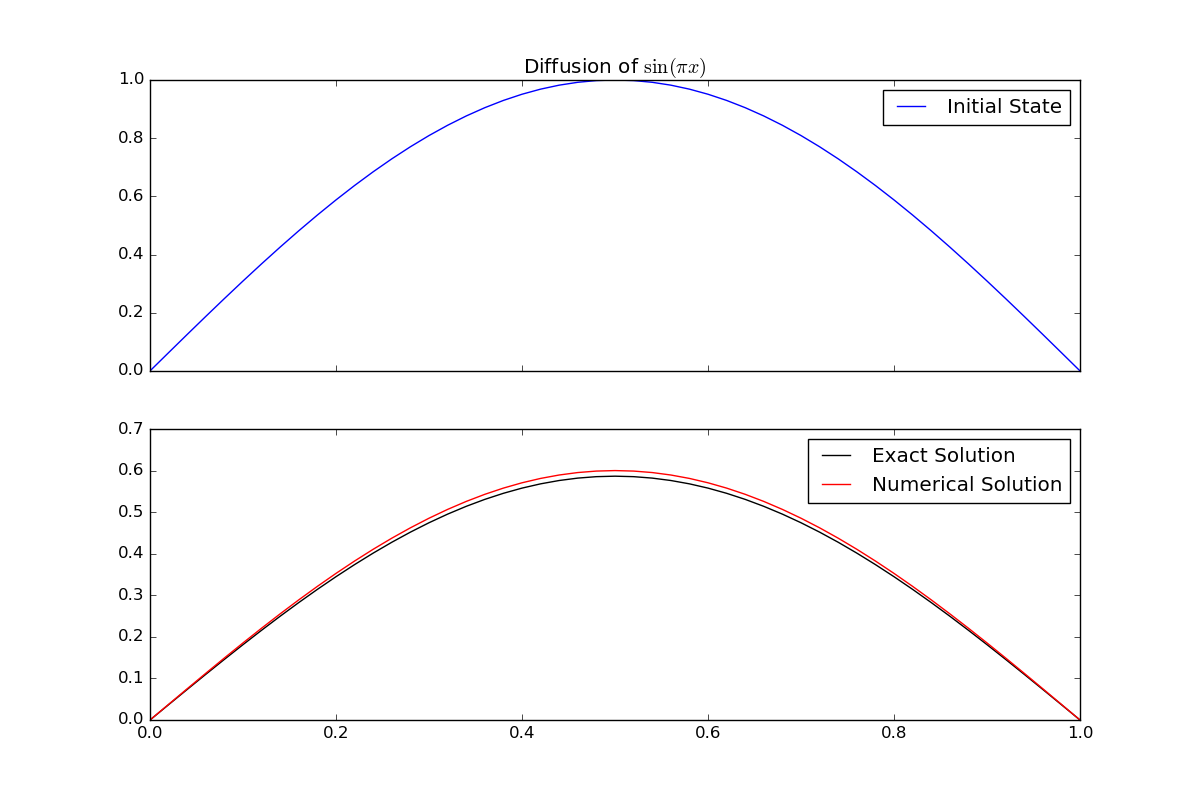
\includegraphics[width=\linewidth]{diffusion.png}
  \caption{
    The diffusion of a simple sinusoid. The pulse is simply spread out
    and the peak falls.
  }
  \label{fig:diffusion}
\end{figure}

\subsubsection{The Advection-Diffusion Equation}

By combining the two previous sections on advection and diffusion, the
advection-diffusion equation is:
\begin{equation}
  u_t = \beta u_xx - c u_x
\end{equation}
where the initial condition is advected with speed $c$ and diffusing
with rate $\beta$. The finite difference equation, stepping forward in
time, using the centred difference scheme for the second derivative
and backward for the first derivative, is:
\begin{equation}
  \frac{u_j^{n+1} - u_j^n}{\Delta t} = \beta \frac{u_{j+1}^n + 2 u_j^n
    + u_{j-1}^n}{\Delta x^2} - c \frac{u_j^n - u_{j-1}^n}{\Delta x}
\end{equation}

The von Neumann stability analysis is done similarly to before,
subsituting $u_j^n = G^n e^{i k j \Delta x}$ and solving for $G^1$:
\begin{equation}
  \begin{aligned}
    e^{i k j \Delta x} \frac{G^{n+1} - G^n}{\Delta t} &=
    \beta G^n \frac{e^{i k (j + 1) \Delta x} - 2 e^{i k j \Delta x}
      + e^{i k (j - 1) \Delta x}}{\Delta x^2} \\
    &- c G^n \frac{e^{i k j \Delta x}
      e^{i k (j - 1) \Delta x}}{\Delta x} \\
    \frac{G^1 - 1}{\Delta t} &= \beta \frac{e^{i k \Delta x} - 2 +
      e^{- i k \Delta x}}{\Delta x^2} \\
    &- c \frac{1 - e^{- i k \Delta
        x}}{\Delta x} \\
    \therefore G^1 &= 1 + 2 s \left( \cos(k \Delta x) - 1 \right) \\
    &+ r \left(e^{-i k \Delta x} - 1 \right)
  \end{aligned}
\end{equation}
Looking at the extreme values of $G^1$ and imposing the stability
condition $|G^1| \leq 1$, the upper extreme when $\cos(k \Delta x) =
1$ results in $|G^1| = 1$. On the lower extreme, when $\cos(k \Delta x
= -1$, the condition is:
\begin{equation}
  \begin{aligned}
    -1 &\leq 1 - 4s - 2r =1 - 2 \Delta t \left( \frac{2 \beta}{\Delta
        x^2} + \frac{2 c}{\Delta x} \right) \\
    \therefore \Delta t &\leq \Delta t_{max} = \frac{\Delta x^2}{c
      \Delta x + 2 \beta}
  \end{aligned}
\end{equation}

This time, the grid has $101$ points, $c = 0.5$, $\beta = 0.1$,
$\Delta t = 0.9 \Delta t_{max}$, and the solution is run until $t =
57$s, shown in figure \ref{fig:advec_diffuse}. The entire simulation
took $2277$ time steps. The behaviour is a combination of what was
observed in the advection equation, since the peak has moved from
$x=0.5$ to $x=0.61$, while the height of the peak has also decreased,
resulting from the diffusion.

\begin{figure}
  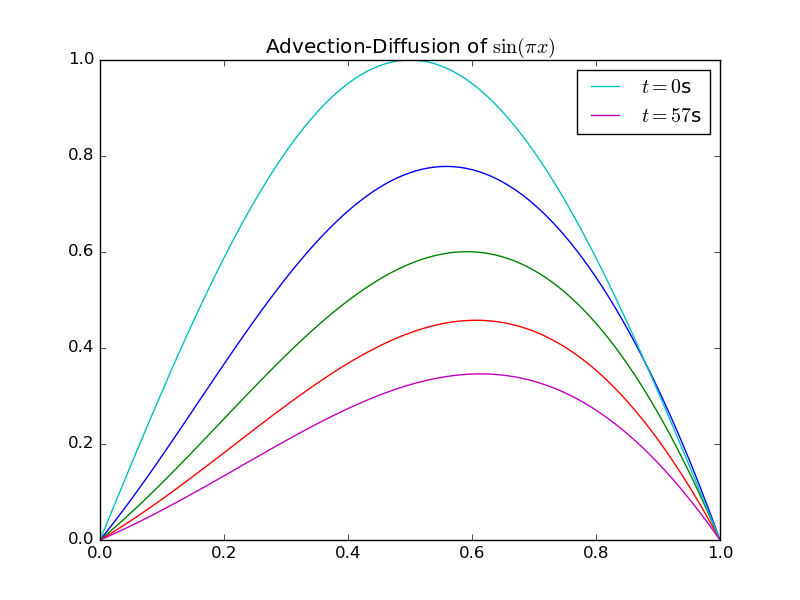
\includegraphics[width=\linewidth]{advection_diffusion.png}
  \caption{
    The advection-diffusion equation applied on a simple
    sinusoid. This is a combination of the advection and diffusion
    behaviour observed in the previous two parts.
  }
  \label{fig:advec_diffuse}
\end{figure}

\section{Discussion}

The sections on the advection-diffusion serve to show the importance
of the CFL conditions and the effect they have on the various schemes
used to step forward in time. In general, the implicit methods
(backward Euler and Crank-Nicholson) were more stable, even as the
Courant number was increased to be over $1$. However, the implicit
methods were also observed to exhibit high frequency oscillations at
the boundary and from sharp abrupt changes in slope. Von Neumann
stability analysis proved to be a reliable way to define an
appropriate size for the time step.

% I'm not sure what else to say about how it relates to the other
% parts, but that's the gist of it.

\end{document}